%%%%%%%%%%%%%%%%%%%%%%%%%%%%%%%%%%%%%%%%%%%%%%%%%%%%%%%%%%%%%%%%%%%%%%
% Overleaf (WriteLaTeX) Example: Molecular Chemistry Presentation
%
% Source: http://www.overleaf.com
%
% In these slides we show how Overleaf can be used with standard
% chemistry packages to easily create professional presentations.
%
% Feel free to distribute this example, but please keep the referral
% to overleaf.com
%
%%%%%%%%%%%%%%%%%%%%%%%%%%%%%%%%%%%%%%%%%%%%%%%%%%%%%%%%%%%%%%%%%%%%%%

\documentclass[xcolor={dvipsnames}]{beamer}

\mode<presentation>
{
  \usetheme{Madrid}       % or try default, Darmstadt, Warsaw, ...
  \usecolortheme{default} % or try albatross, beaver, crane, ...
  \usefonttheme{default}    % or try default, structurebold, ...
  \setbeamertemplate{navigation symbols}{}
  \setbeamertemplate{caption}[numbered]
}

\usepackage[english]{babel}
\usepackage[utf8x]{inputenc}
\usepackage{graphicx}
\usepackage{hyperref}
  \hypersetup{colorlinks=true}
  \hypersetup{urlcolor=blue}
  \hypersetup{linkcolor = .}
\usepackage{xcolor}
\usepackage{siunitx}
  \sisetup{separate-uncertainty = true}
\DeclareSIUnit\barn{b}
\usepackage{physics}
\usepackage[font=small,labelfont=bf]{caption}
\usepackage{subcaption}
\usepackage[en-GB]{datetime2}
\usepackage{overpic}
\usepackage{feynmp}
\DeclareGraphicsRule{*}{mps}{*}{}
\usepackage{scalerel}
\newcommand{\mylbrace}[2]{\vspace{#2pt}\hspace{6pt}\scaleleftright[\dimexpr5pt+#1\dimexpr0.06pt]{\lbrace}{\rule[\dimexpr2pt-#1\dimexpr0.5pt]{-4pt}{#1pt}}{.}}
\newcommand{\myrbrace}[2]{\vspace{#2pt}\scaleleftright[\dimexpr5pt+#1\dimexpr0.06pt]{.}{\rule[\dimexpr2pt-#1\dimexpr0.5pt]{-4pt}{#1pt}}{\rbrace}\hspace{6pt}}

% Trim in percent
\usepackage{adjustbox}

% No "Figure" prefix
\setbeamertemplate{caption}{\raggedright\insertcaption\par}

% Nice decay amplitude diagrams
\usepackage{amsmath,amssymb,tikz-cd}

% Strike out text
\usepackage[normalem]{ulem}

% For figures with text overlay
\usepackage{overpic}

% Arrows
\usepackage{tikz}
\newcommand{\tikzmark}[1]{\tikz[remember picture] \node[coordinate] (#1) {#1};}

% Colourbox with line breaks
\newcommand{\cbox}[2][lime!20]{%
  \colorbox{#1}{\parbox{\dimexpr\linewidth-2\fboxsep}{\strut #2\strut}}%
}

% Vector arrows
\usepackage[pdftex]{pict2e}

% Checkmark symbol
\def\checkmark{\tikz\fill[scale=0.4](0,.35) -- (.25,0) -- (1,.7) -- (.25,.15) -- cycle;}

% Here's where the presentation starts, with the info for the title slide
\title[Tracking efficiency meeting]{Update on 2025 and 2026 tracking efficiencies}

\author[Martin Tat]{Martin Tat}
\institute[Heidelberg]{Heidelberg University}
\date{2nd June 2026}

\titlegraphic{
\includegraphics[height = 2.3cm]{lhcb.jpg}\hspace{1.0cm}~%
              
\includegraphics[height = 2.3cm]{HeidelbergLogo.pdf}}

\begin{document}

\begin{frame}
  \titlepage
\end{frame}

% These three lines create an automatically generated table of contents.
%\begin{frame}{Outline}
%  \tableofcontents
%\end{frame}

\begin{frame}{Progress update}
  \vspace{0.0cm}
  {\large Progress update:}
  \vspace{0.2cm}
  \begin{enumerate}
    \setlength\itemsep{0.8em}
    \item{Tracking efficiency tables produced for 2025 block 1 and 2 (pre-TS)}
    \begin{itemize}
      \item[-]{Velo M23 turned off in MC, but not in data}
    \end{itemize}
    \item{Tracking efficiencies fitted to all of 2025 and 2026 data using 2025 pre-TS MC to constrain fit shapes}
    \begin{itemize}
      \item[-]{Radiation damage in the central region visible}
      \item[-]{Damaged Velo clearly visible in highest $\eta$ bin and high momentum}
      \item[-]{Runs with muon hole checked}
    \end{itemize}
    \item{Plan to present in RTA WP4 on Thursday}
    \item{MC request for 2025 post-TS approved, delayed because MC liason was away}
  \end{enumerate}
\end{frame}

\begin{frame}{2025 pre-TS tracking efficiency corrections}
  \vspace{0.0cm}
  \begin{figure}[htb]
    \centering
    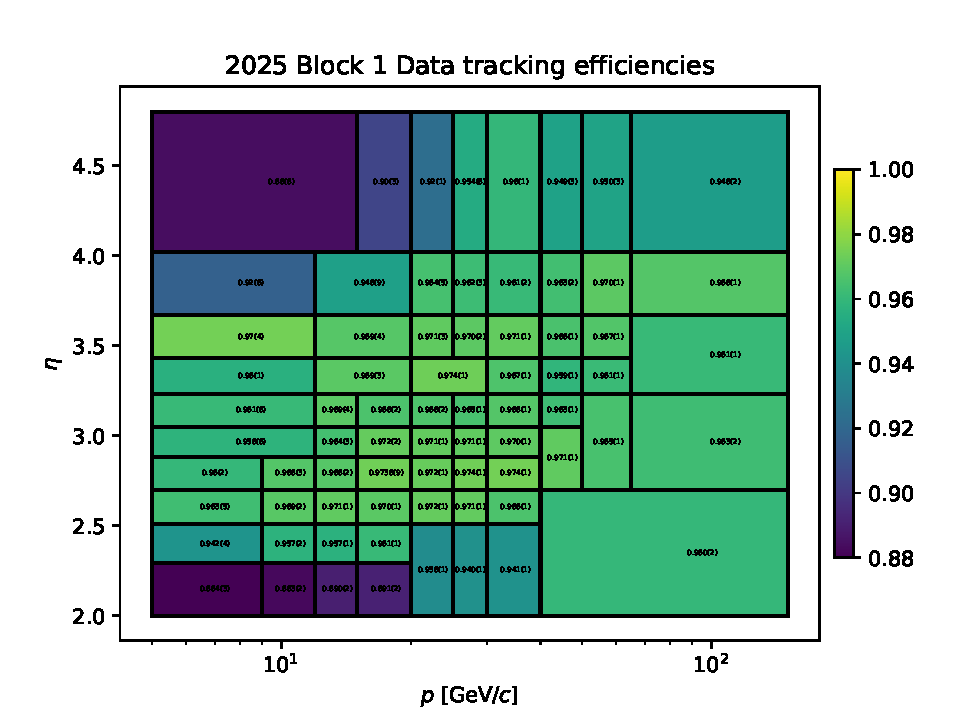
\includegraphics[width=0.85\textwidth]{Plots/TrackingEfficiencies_2D_binning_2025_Block1_Data_colour.pdf}
  \end{figure}
\end{frame}

\begin{frame}{2025 pre-TS tracking efficiency corrections}
  \vspace{0.0cm}
  \begin{figure}[htb]
    \centering
    
\includegraphics[width=0.85\textwidth]{Plots/TrackingEfficiencies_2D_binning_2025_Block1_MC_colour.pdf}
  \end{figure}
\end{frame}

\begin{frame}{2025 pre-TS tracking efficiency corrections}
  \vspace{0.0cm}
  \begin{figure}[htb]
    \centering
    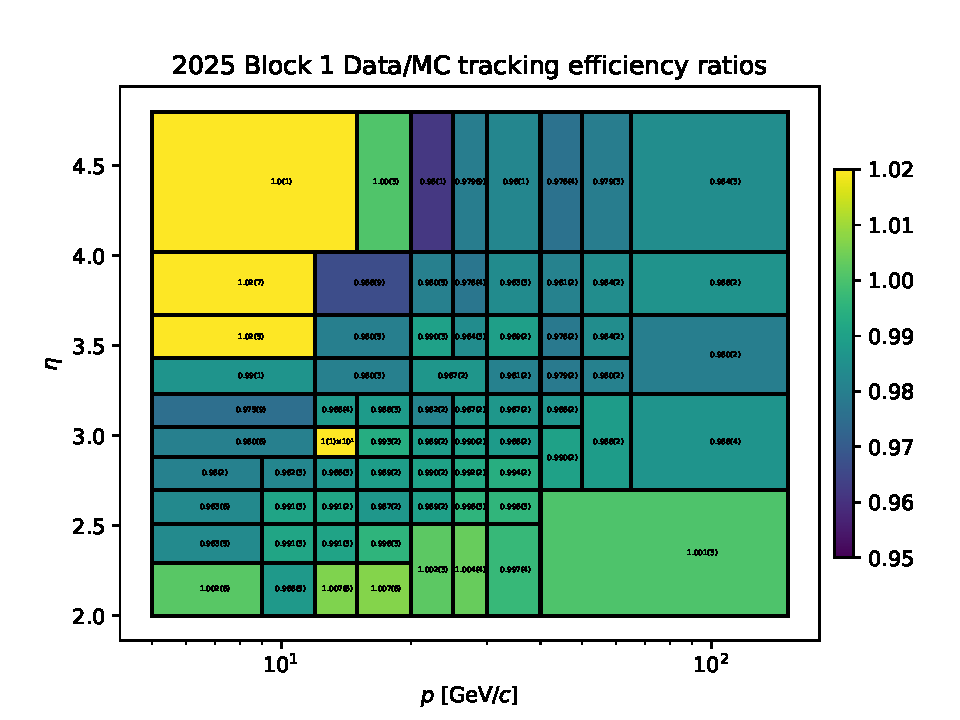
\includegraphics[width=0.85\textwidth]{Plots/TrackingEfficiencies_2D_binning_2025_Block1_Ratio_colour.pdf}
  \end{figure}
\end{frame}

\begin{frame}{2025 pre-TS tracking efficiency corrections}
  \vspace{0.0cm}
  \begin{figure}[htb]
    \centering
    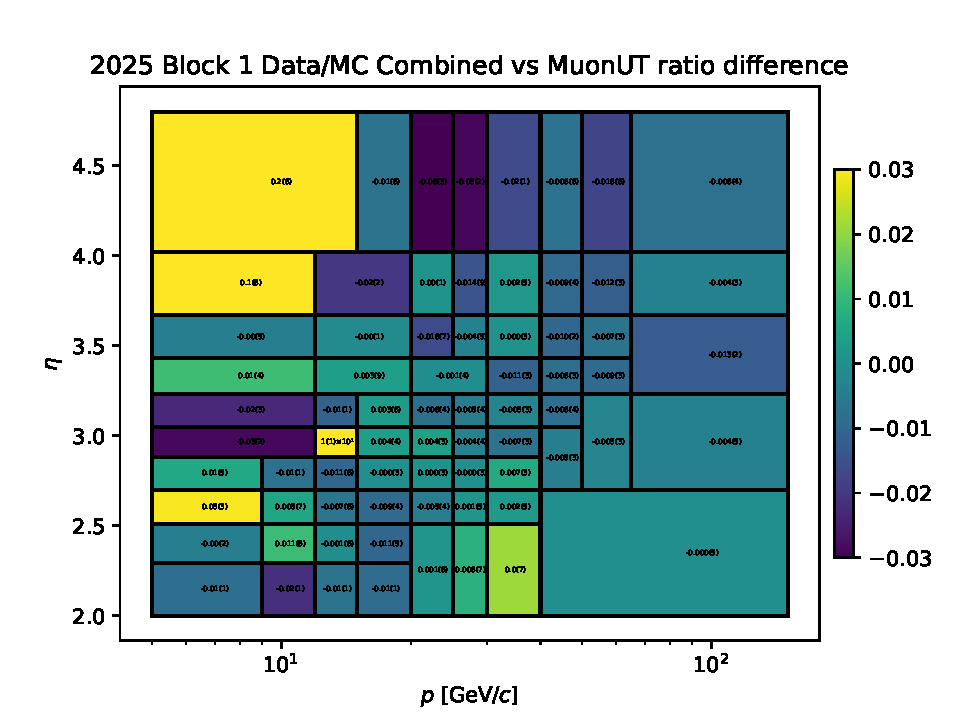
\includegraphics[width=0.85\textwidth]{Plots/TrackingEfficiencies_2D_binning_2025_Block1_RatioDiff_colour.pdf}
  \end{figure}
\end{frame}

\begin{frame}{2025 pre-TS tracking efficiency corrections}
  \vspace{0.0cm}
  \begin{figure}[htb]
    \centering
    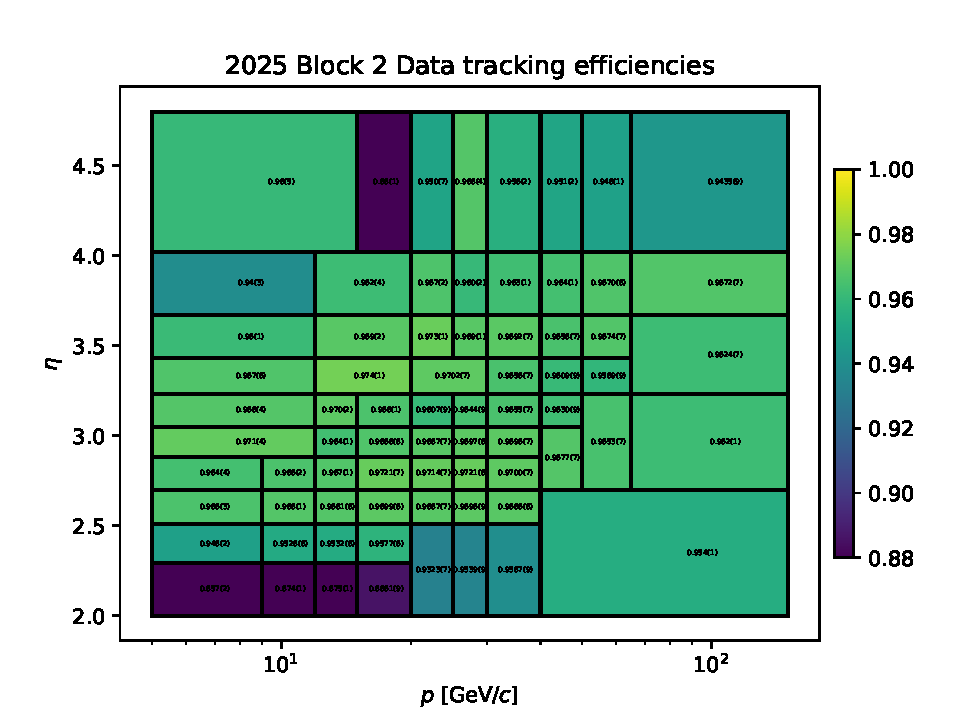
\includegraphics[width=0.85\textwidth]{Plots/TrackingEfficiencies_2D_binning_2025_Block2_Data_colour.pdf}
  \end{figure}
\end{frame}

\begin{frame}{2025 pre-TS tracking efficiency corrections}
  \vspace{0.0cm}
  \begin{figure}[htb]
    \centering
    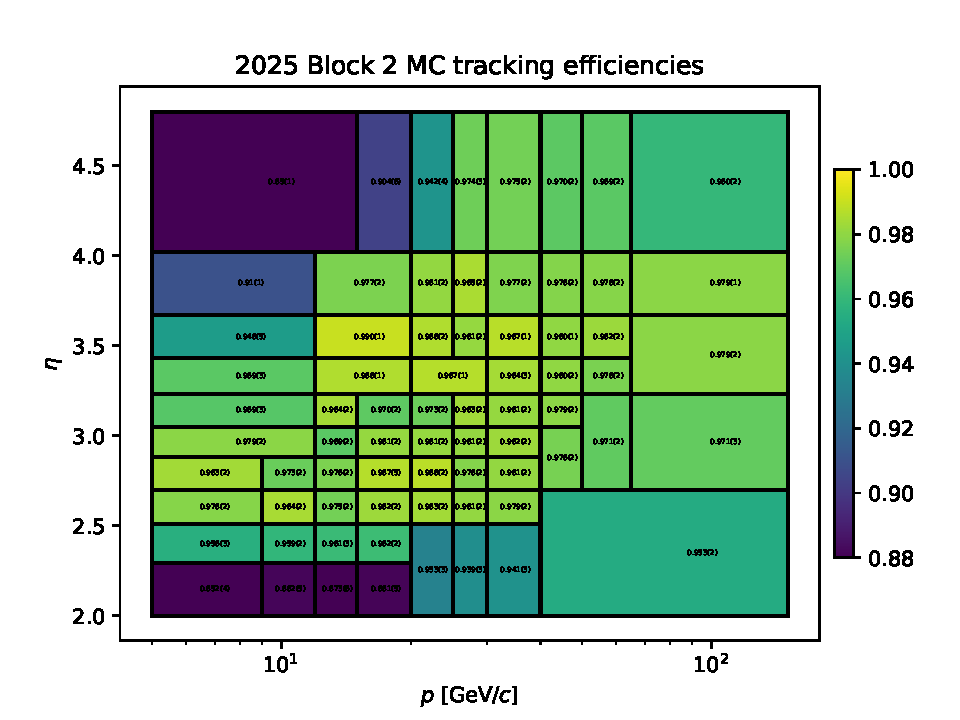
\includegraphics[width=0.85\textwidth]{Plots/TrackingEfficiencies_2D_binning_2025_Block2_MC_colour.pdf}
  \end{figure}
\end{frame}

\begin{frame}{2025 pre-TS tracking efficiency corrections}
  \vspace{0.0cm}
  \begin{figure}[htb]
    \centering
    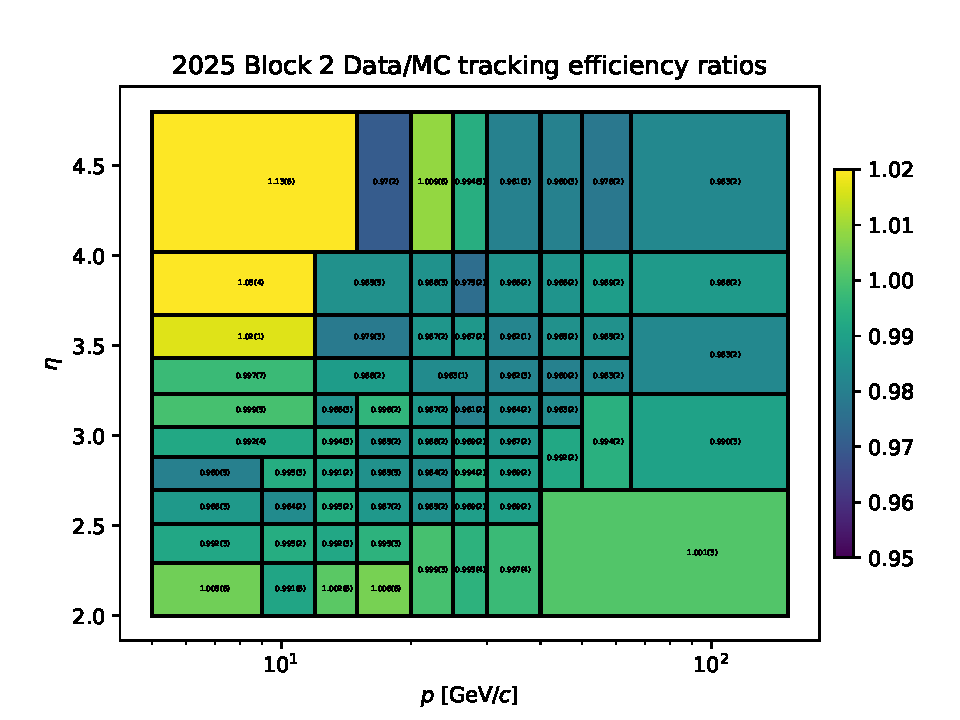
\includegraphics[width=0.85\textwidth]{Plots/TrackingEfficiencies_2D_binning_2025_Block2_Ratio_colour.pdf}
  \end{figure}
\end{frame}

\begin{frame}{2025 pre-TS tracking efficiency corrections}
  \vspace{0.0cm}
  \begin{figure}[htb]
    \centering
    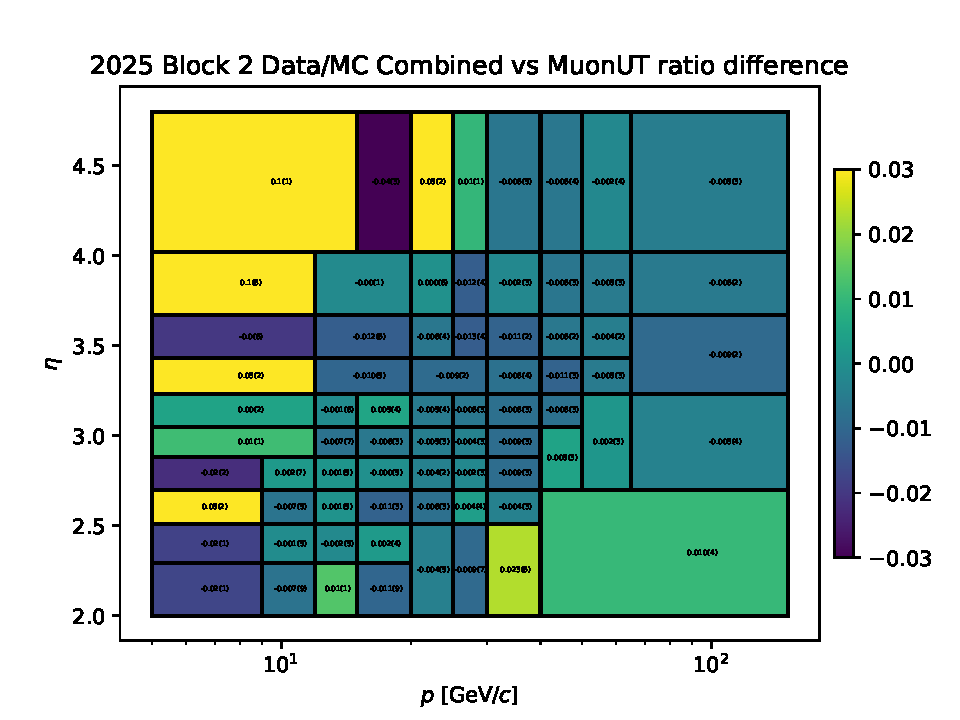
\includegraphics[width=0.85\textwidth]{Plots/TrackingEfficiencies_2D_binning_2025_Block2_RatioDiff_colour.pdf}
  \end{figure}
\end{frame}

\begin{frame}{2025 and 2026 data tracking efficiencies}
  \vspace{0.0cm}
  {\large Comparison of tracking efficiencies in 2025 and 2026 data blocks}
  \begin{figure}[htb]
    \centering
    \begin{subfigure}{0.5\textwidth}
      \centering
      
\includegraphics[width=1.0\textwidth]{Plots/trackeff_Data_VeloMuon_P_workdir_samples.pdf}
    \end{subfigure}%
    \begin{subfigure}{0.5\textwidth}
      \centering
      
\includegraphics[width=1.0\textwidth]{Plots/trackeff_Data_VeloMuon_ETA_workdir_samples.pdf}
    \end{subfigure}
  \end{figure}
  {VeloMuon track efficiencies\\Looks like radiation damage in the central region}
\end{frame}

\begin{frame}{2025 and 2026 data tracking efficiencies}
  \vspace{0.0cm}
  {\large Comparison of tracking efficiencies in 2025 and 2026 data blocks}
  \begin{figure}[htb]
    \centering
    \begin{subfigure}{0.5\textwidth}
      \centering
      
\includegraphics[width=1.0\textwidth]{Plots/trackeff_Data_Downstream_P_workdir_samples.pdf}
    \end{subfigure}%
    \begin{subfigure}{0.5\textwidth}
      \centering
      
\includegraphics[width=1.0\textwidth]{Plots/trackeff_Data_Downstream_ETA_workdir_samples.pdf}
    \end{subfigure}
  \end{figure}
  {Downstream track efficiencies\\Velo damage at the end of 2025 clearly seen!}
\end{frame}

\begin{frame}{Muon hole in 2026 data tracking efficiencies}
  \vspace{0.0cm}
  {\large Check tracking efficiencies in CONDITIONAL runs with muon hole (\href{https://lbproblems.cern.ch/problemdb/problems/1081/}{see here})}
  \begin{figure}[htb]
    \centering
    \begin{subfigure}{0.5\textwidth}
      \centering
      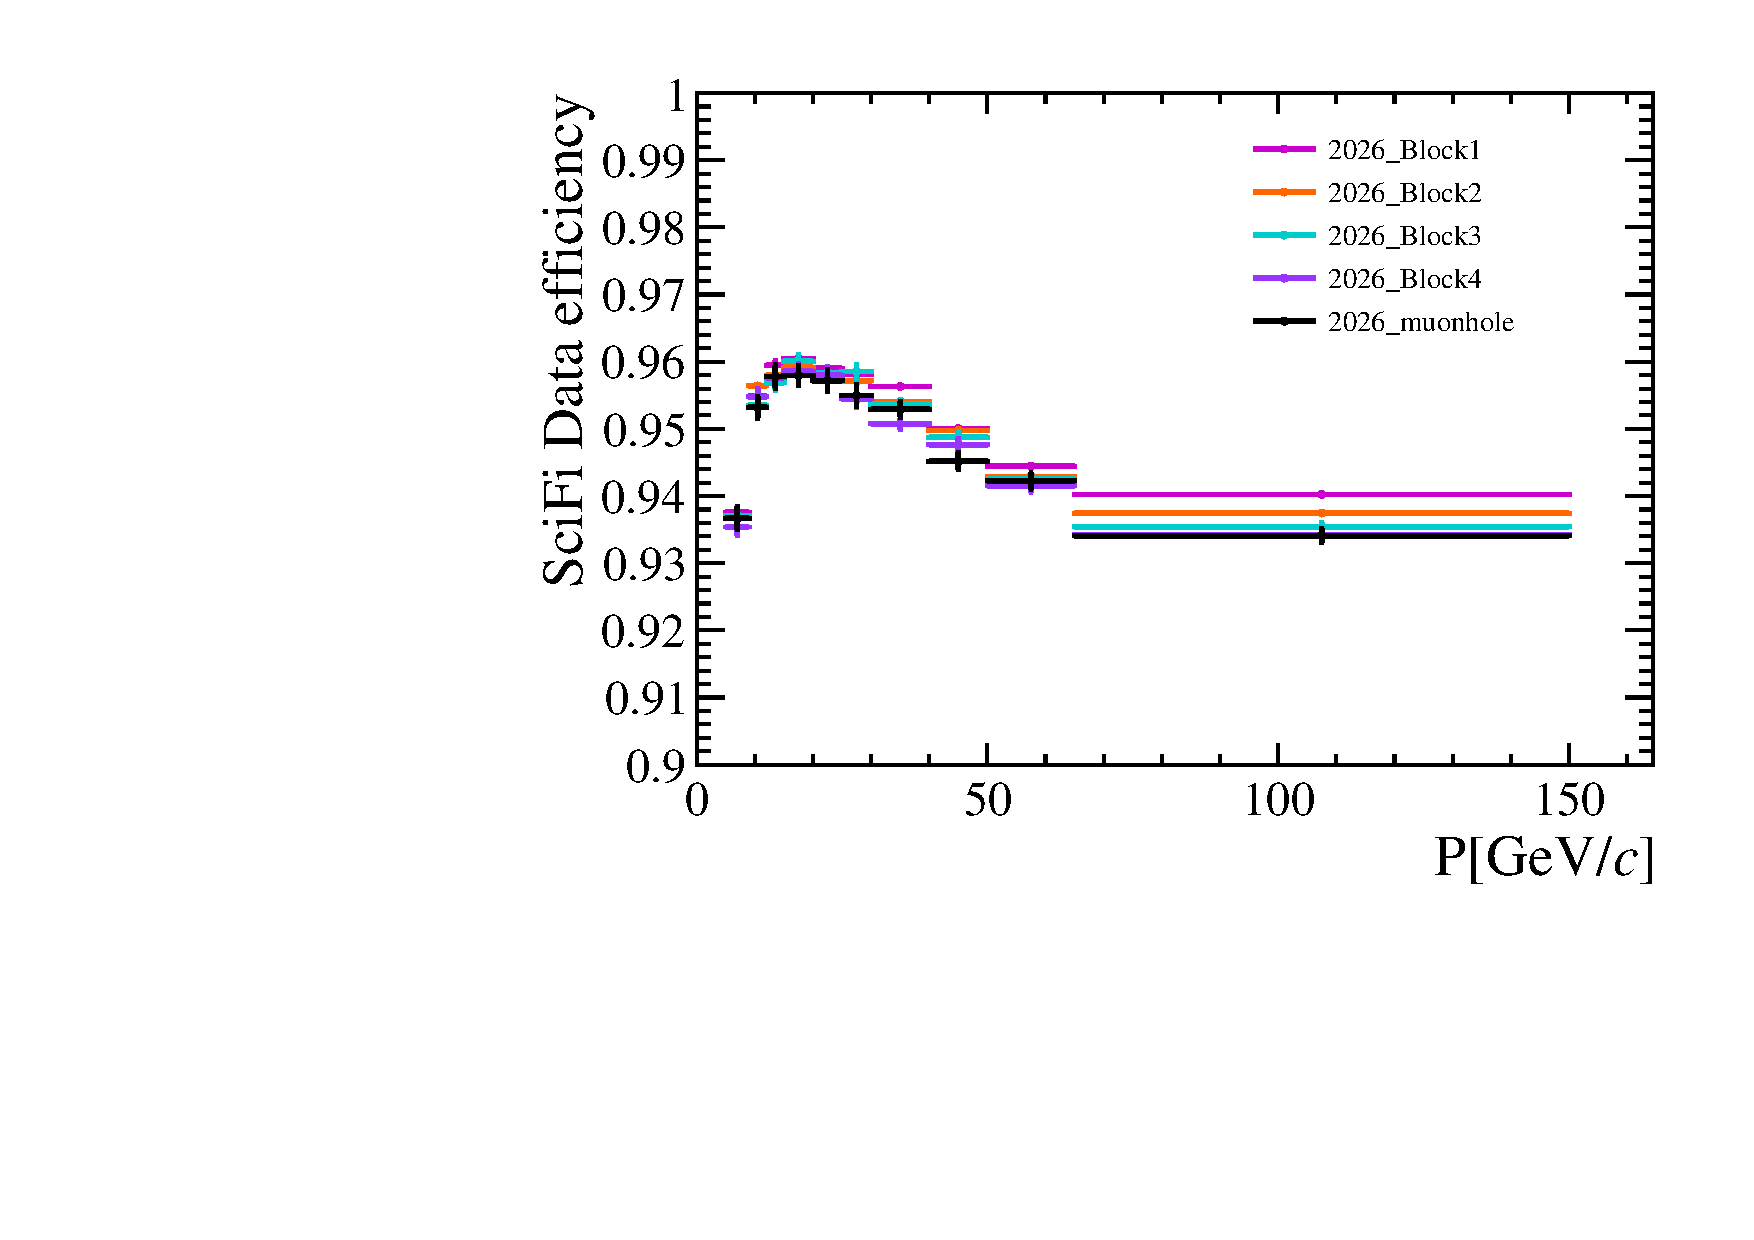
\includegraphics[width=1.0\textwidth]{Plots/trackeff_Data_VeloMuon_P_muonhole_samples.pdf}
    \end{subfigure}%
    \begin{subfigure}{0.5\textwidth}
      \centering
      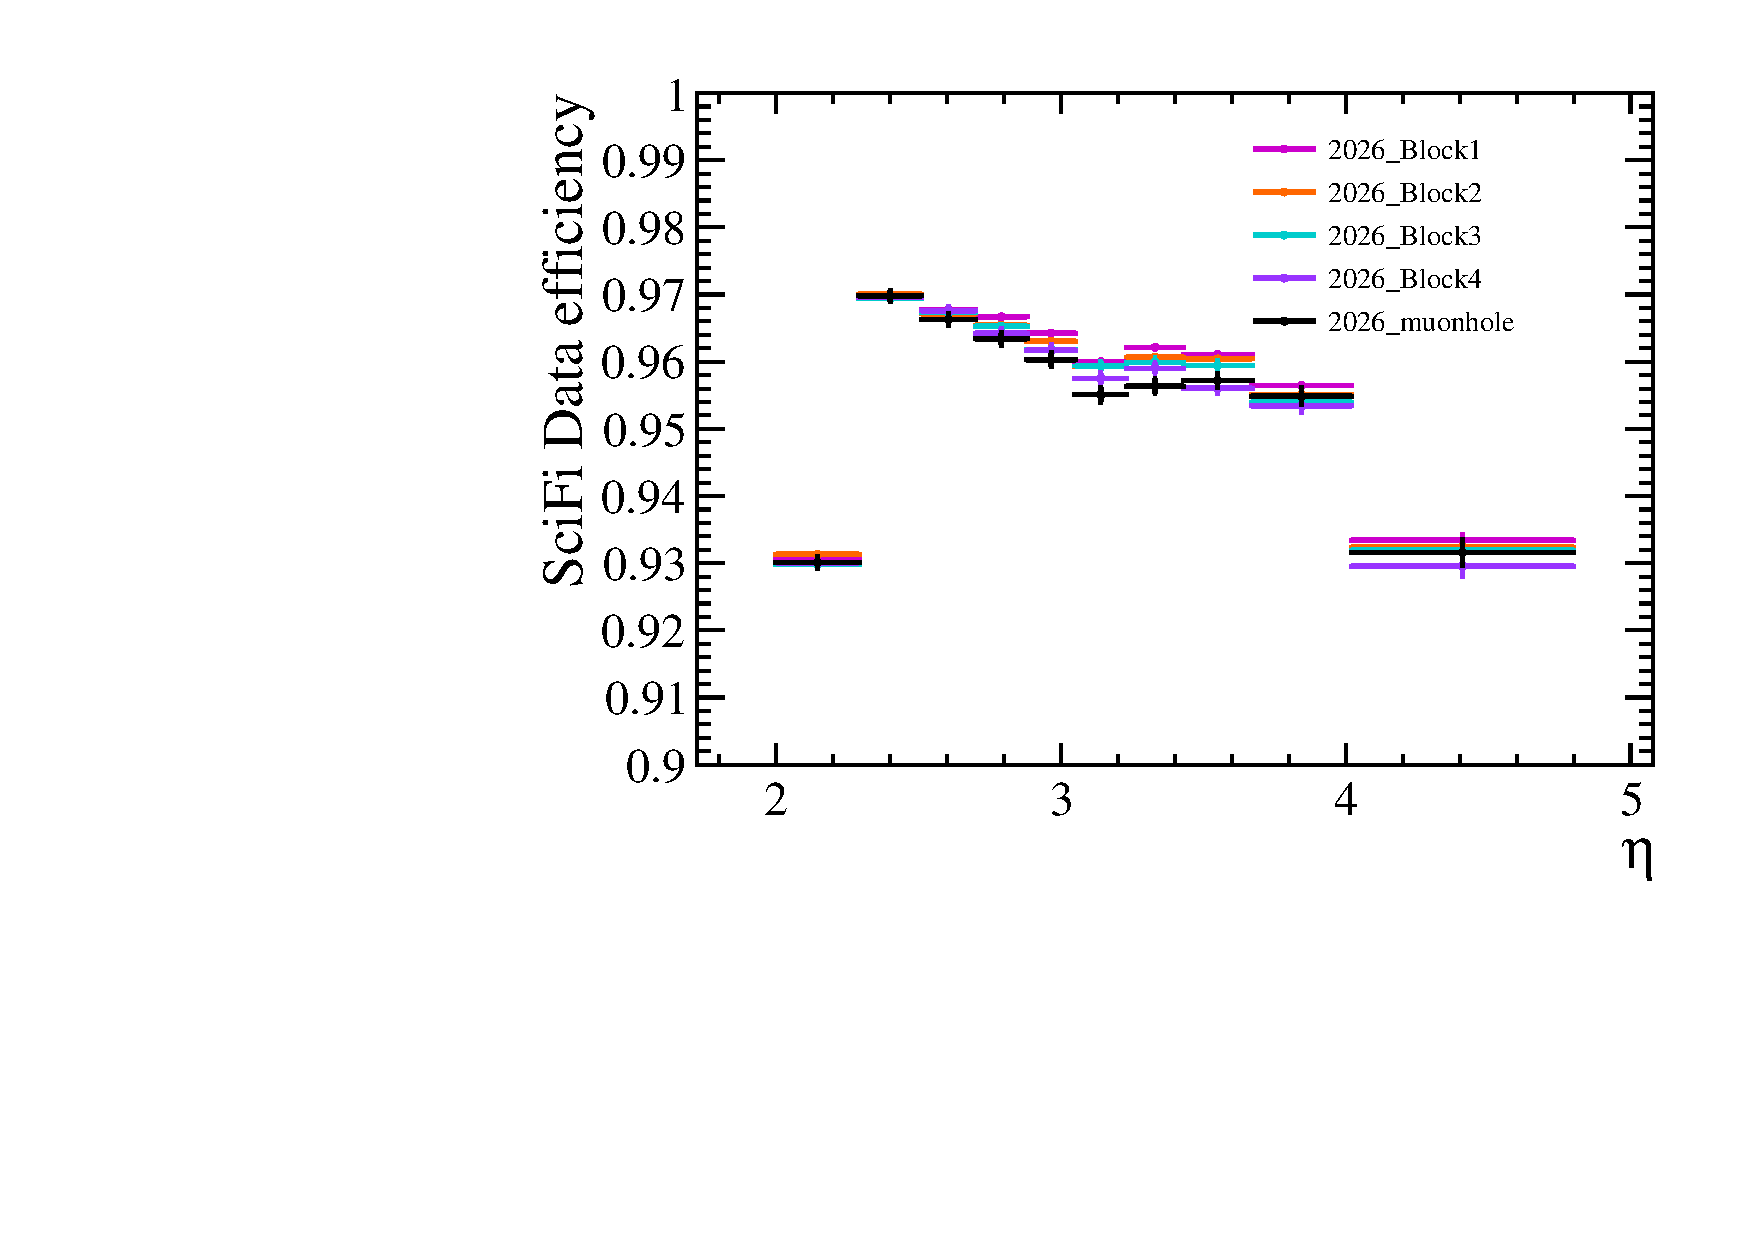
\includegraphics[width=1.0\textwidth]{Plots/trackeff_Data_VeloMuon_ETA_muonhole_samples.pdf}
    \end{subfigure}
  \end{figure}
  {VeloMuon track efficiencies\\Maybe small drop near $\eta\approx3.5$}
\end{frame}

\begin{frame}{Muon hole in 2026 data tracking efficiencies}
  \vspace{0.0cm}
  {\large Check tracking efficiencies in CONDITIONAL runs with muon hole (\href{https://lbproblems.cern.ch/problemdb/problems/1081/}{see here})}
  \begin{figure}[htb]
    \centering
    \begin{subfigure}{0.5\textwidth}
      \centering
      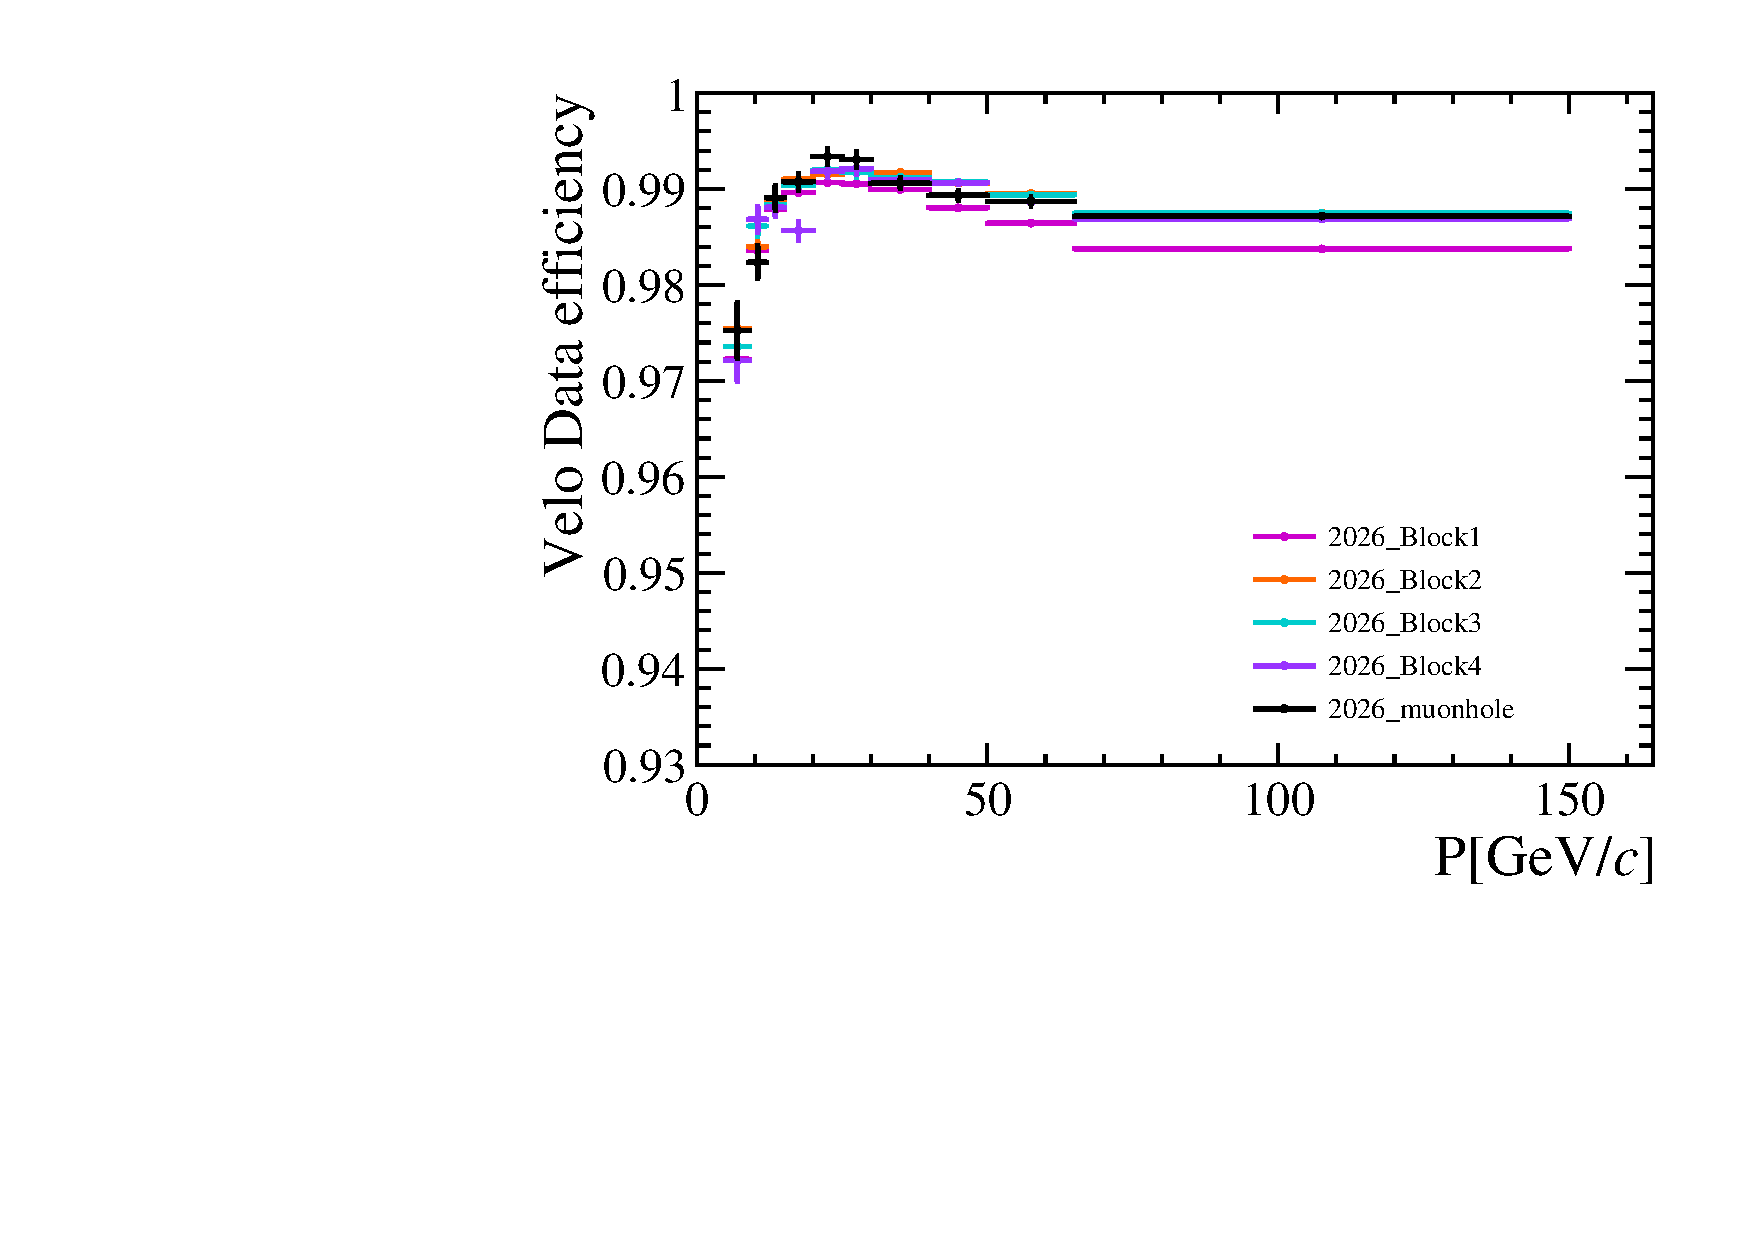
\includegraphics[width=1.0\textwidth]{Plots/trackeff_Data_Downstream_P_muonhole_samples.pdf}
    \end{subfigure}%
    \begin{subfigure}{0.5\textwidth}
      \centering
      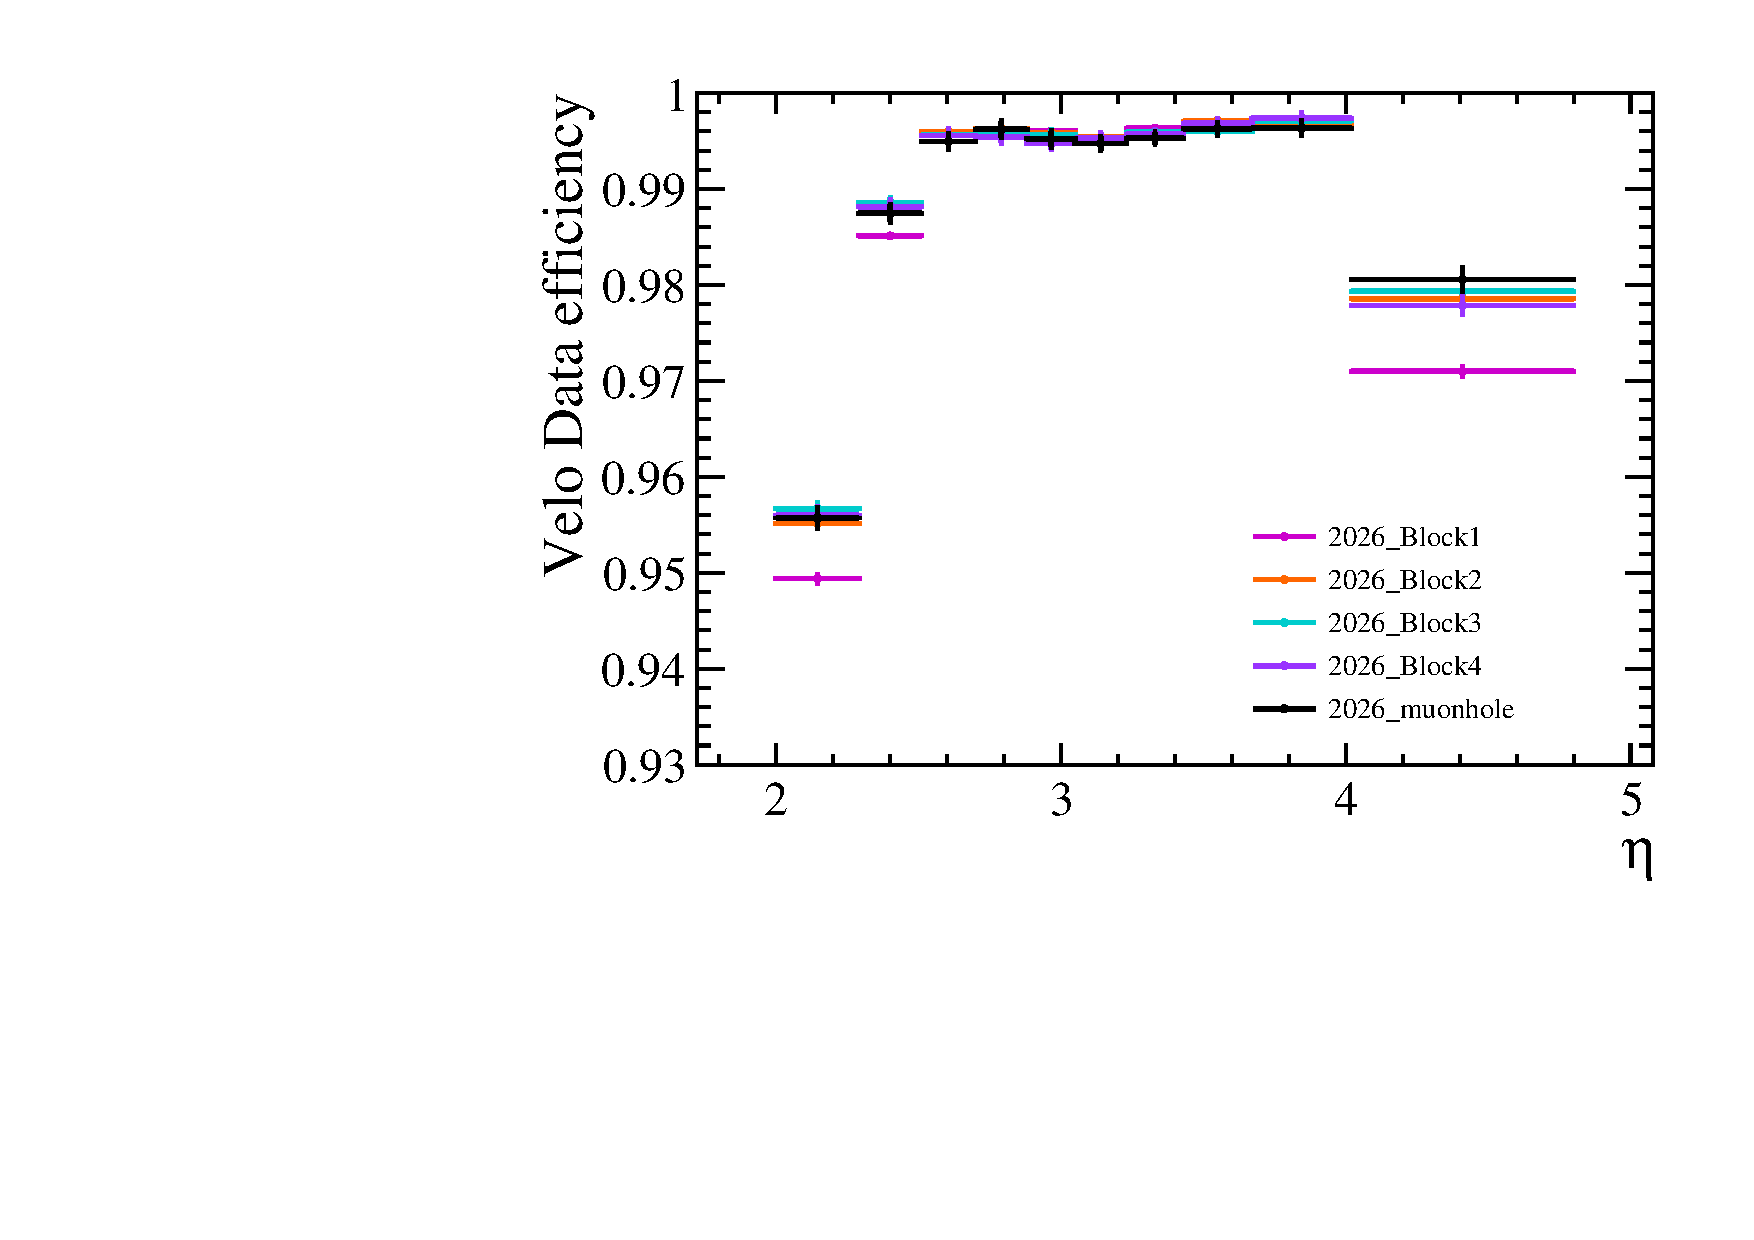
\includegraphics[width=1.0\textwidth]{Plots/trackeff_Data_Downstream_ETA_muonhole_samples.pdf}
    \end{subfigure}
  \end{figure}
  {Downstream track efficiencies\\No effect seen!}
\end{frame}

\begin{frame}{Binning in Velo halves}
  \vspace{0.0cm}
  {\large Issue raised last time:}
  \vspace{0.2cm}
  \begin{itemize}
    \setlength\itemsep{0.8em}
    \item{We need to bin the two Velo halves separately...}
    \item{...but which variable to use?}
    \item{\texttt{PHI} is most convenient for analysts}
    \item{\texttt{NVPHITSA/C} functors gives the number of hits in each Velo half}
    \item{I did a quick quantitative study: When binning in \texttt{PHI}, around $15\%$--$18\%$ of tracks are assigned the wrong Velo half}
    \item{\texttt{NVPHITSA/C} can also be ambigious, happens for $3\%$ of the tracks in VeloMuon}
    \item{But in Downstream, Velo hits are not defined for the probe track, and I don't think it makes sense to use the Velo hits of the best matched track if it's not matched...?}
  \end{itemize}
\end{frame}

\begin{frame}{Plan next}
  \vspace{0.0cm}
  {\large Not much to do for now:}
  \vspace{0.2cm}
  \begin{enumerate}
    \setlength\itemsep{0.8em}
    \item{Wait for large 2024 MC production}
    \item{Wait for 2025 post-TS MC}
  \end{enumerate}
\end{frame}

\end{document}
